\documentclass[10pt]{article}
\textwidth 16.5cm
\textheight 23.5cm
\oddsidemargin 0pt
\topmargin -2cm
% \usepackage{epsf}

% Draft watermark
\usepackage[
stamp = true,
firstpageonly = true
]{draftwatermark}

% Font and formatting
\usepackage[default]{lato}
\usepackage[skip=3pt]{parskip}
\usepackage{titlesec}
\titlespacing{\paragraph}{0pt}{*1}{*2}

% \usepackage[compact]{titlesec} 


% Writing maths
\usepackage{
    amsmath, % aligns, equations, etc.
    amsfonts, % blackboard bold, etc.
    bbm, % blackboard bold for numbers.
}

% Figures
\usepackage{graphicx}
\usepackage{floatrow}
\floatsetup[table]{capposition=top}
\newcommand*{\figuretitle}[1]{%
    {\centering%   <--------  will only affect the title because of the grouping (by the
    \textbf{#1}%              braces before \centering and behind \medskip). If you remove
    \par\medskip}%            these braces the whole body of a {figure} env will be centered.
}

% Boxes
\usepackage{tcolorbox}
\definecolor{edi-dark-purple}{rgb}{0.4882812,0.046875,0.4296875}
\definecolor{edi-light-purple}{rgb}{0.9453125,0.8359375,0.9140625}

% References
\usepackage[
    colorlinks,
    linkcolor=black,
    citecolor=edi-dark-purple, 
    urlcolor=edi-dark-purple,
    breaklinks = true
]{hyperref}
\usepackage{xurl}
\usepackage[sort&compress, numbers]{natbib}
\bibliographystyle{unsrtnat}
\usepackage{multicol}
\renewcommand{\bibpreamble}{\begin{multicols}{2}}
\renewcommand{\bibpostamble}{\end{multicols}}

% Acronyms
\usepackage[acronym, toc]{glossaries-extra}

\setabbreviationstyle[acronym]{long-short}
\glssetcategoryattribute{acronym}{nohyperfirst}{true}
\renewcommand*{\glsdonohyperlink}[2]{%
 {\glsxtrprotectlinks \glsdohypertarget{#1}{#2}}}

 \newacronym{bfo}{BFO}{Border Force Officer}
 \newacronym[plural=SLAs, firstplural=Service Level Agreements]{sla}{SLA}{Service Level Agreement}
 \newacronym[plural=eGates, firstplural=electronic passport Gates]{egate}{eGate}{electronic passport Gate}
 \newacronym[plural=KPIs, firstplural=Key Performance Indicators]{kpi}{KPI}{Key Performance Indicator}

% Inline comments from Jacob and Bella
\usepackage{xcolor}
\usepackage[draft,inline,nomargin,index]{fixme}
\fxsetup{theme=color,mode=multiuser}
\FXRegisterAuthor{jb}{ajb}{\color{blue} JB}
\FXRegisterAuthor{bd}{abd}{\color{red} BD}

\title{Planning for Future Demand on Border Operations\\ at Edinburgh Airport}
 \author{Isabella Deutsch and Jacob R. Bradley}
 \date{}


\begin{document}
\maketitle

\section{Introduction}
A large number of passengers arriving internationally at Edinburgh Airport need to pass through immigration. These passengers are either processed at a desk staffed by a \gls{bfo} or, for passengers of certain nationalities, at an automated \gls{egate}. With overall passenger footfall expected to increase substantially over the next five years, pressure on immigration services is also growing, and the airport will need to adapt its operations in order to accommodate its international arrivals safely and efficiently. In particular, the airport has committed to several \glspl{sla} ensuring quality of experience for arrivals. One avenue being explored to meet \glspl{sla} under increased demand is the expanded use of \glspl{egate}, both through additional construction and measures encouraging increased uptake \cite{UK_border_2025}. In this report we investigate the outcomes of these measures, providing clear recommendations for \gls{egate} construction over the next five years (2023-2027). For key results, see our one page high-level summary. To explore \gls{egate} construction and usage scenarios interactively, see our \href{https://github.com/cobrbra/immigration_queue_simulation_edinburgh_airport}{Shiny App}.
% This does not apply for anyone arriving from the United Kingdom (including Northern Ireland), the Crown Dependencies, and the Republic of Ireland, as there are no routine passport controls between these countries \cite{common_travel_area}.
% Only passengers of certain nationality are eligible to use the \glspl{egate}, as defined below. There are currently 9 desks and 10 \glspl{egate} in operation at Edinburgh Airport. 

\subsection{Problem Statement}
The task set by Edinburgh Airport is to develop a simulation model of immigration queuing that can be used to test a variety of demand scenarios, including overall and demographic changes in passenger arrivals, process enhancements, and increased \gls{egate} availability. 
Additionally, sensitivity analysis is required to assess the robustness of these recommendations under a variety of scenarios.
The overall performance of Edinburgh Airport's immigration queuing operation is measured via three \glspl{kpi} and their related \glspl{sla}, defined below.

\subsection{Key Performance Indicators}

Three \glspl{kpi} have been identified to evaluate the airport's immigration queue process, defined as follows.

\begin{itemize}
    \item \textbf{Queue length(s)}: The number of passengers queuing for a desk or \gls{egate} in the immigration hall/overflow zones at any given time.
    \item \textbf{Wait time}: Time between arrival at the immigration hall/overflow zones and arrival at a desk/\gls{egate} for a given passenger arriving at Edinburgh Airport. 
    \item \textbf{Contingency usage}: Whether immigration hall contingency capacity is in use.
\end{itemize}

We measure \textit{queue length} at evenly spaced time points (typically every 15 minutes). Immigration \textit{wait time}, however, is measured for each arriving passenger. The relationship between queue length and \textit{contingency usage} is determined by the physical division of the immigration hall into desk and \gls{egate} queuing areas.

\subsection{Service Level Agreements}
We consider the following \glspl{sla}, which are derived from \glspl{kpi} and provide targets for passenger experience and operational function. They are set internally and internally by Edinburgh Airport and the UK Border Force. 
\begin{itemize}
    \item \textbf{Proportion of passengers with a wait time less than 15 (or 60) minutes.} \\
    This is in line with the brief and \cite{UK_border_2025}. It is indicative of the experience of individual queuing passengers.
    \item \textbf{Total time using overflow/contingency capacity.} \\
    This describes the impact the queue has on the operations of the airport according to the queuing capacities outlined below. It is measured across a given week of operations. Breach of this \gls{sla} may effect passengers that are not in the immigration queue through disruption of other areas of the airport.
\end{itemize}

\section{Data Sources}
This section outlines the datasets used throughout this report. The majority of the data used for the core components of our analysis were provided by Edinburgh Airport via the Edinburgh SIAM \& IMA Student Chapter Modelling Competition \cite{modelling_competition}. We have made use of several additional external datasets, which are also described here. These are all either in the public domain, or accessible to all researchers participating in the modelling competition. 

\subsection{Competition Data}

We first outline the data received through the modelling competition. This consists of both operational data and the future arrivals schedule and is informed by historic data from Edinburgh Airport.


\subsubsection{Operational Data}

\paragraph{Early and delayed flights}
In the summer of 2019 only 58\% of flights arrived on time (measured if arrived within 15 minutes of scheduled arrival), 21\% were late, and 21\% were early. Of those that were early, average arrival time was 21 minutes ahead of schedule (standard deviation 6 minutes). For late arrivals, average delay was 50 minutes (standard deviation 56 minutes). 

\paragraph{Coached vs contact}
Once an aircraft has reached its parking position there are two ways for passengers to reach the terminal building. \textit{Contact} passengers walk directly from their aircraft to the immigration queue. \textit{Coached} passengers exit the aircraft via stairs and are loaded onto buses, which bring them to the terminal building. The percentage of contact passengers lies around 80\% and varies across years (see Figure~\ref{fig:future_passenger_burden}).

\paragraph{UKIE flights} Flights arriving from the United Kingdom (including Northern Ireland), the Crown Dependencies, and the Republic of Ireland (referred throughout as \textit{UKIE}) do not need to be processed by immigration services, as there are currently no routine passport controls between these countries \cite{common_travel_area}.

\paragraph{eGate eligibility for EU+ passengers}
Passengers of the following nationalities are allowed to use \glspl{egate}: EU countries, Australia, Canada, Iceland, Japan, Liechtenstein, New Zealand, Norway, Singapore, South Korea, Switzerland, and the USA. In the following we refer to these countries as \textit{EU+}. 

\paragraph{Hall capacity}
The immigration hall at Edinburgh Airport has an \textit{initial capacity} for 500 passengers. Its \textit{overflow capacity}, which can be used without overly impacting other areas of the operation, holds a further 150 passengers. There is also \textit{contingency capacity} for an additional 600 passengers. However, its usage negatively impacts the operations of the airport.

\paragraph{Border check transaction times} It takes on average 90 seconds (15 seconds standard deviation) to be processed at a \gls{bfo}-staffed desk. The transaction time at an \gls{egate} is generally shorter with an average of 45 second (5 seconds standard deviation). 

\paragraph{eGate failure rate}
Some passengers who use an \gls{egate} fail to pass through it successfully and need to be processed at a desk instead. This failure rate lies at 9\%.

\subsubsection{Future Arrivals Data} \label{sec:future_arrivals_data}
Via the modelling competition, we have been provided with an anticipated future arrivals schedule and passenger counts for five July weeks (each Monday to Sunday) over the next five years (2023-2027). These comprise a total of 4,123 flights and represent increasing aircraft arrivals over time. These are reflected in an increased passenger throughput over the same time period, comprising increases in both coached and contact arrivals (Figure~\ref{fig:future_passenger_burden}). We are not provided with information on passenger nationalities, or airports of departure. We assume in the following that these do not include UKIE flights. 

% % latex table generated in R 4.2.3 by xtable 1.8-4 package
% Tue Apr 11 11:53:21 2023
\begin{table}[ht]
\centering
\begin{tabular}{cccc}
  \hline
{\textbf{Year}} & {\textbf{Start Date}} & {\textbf{End Date}} & {\textbf{Number of Flights}} \\ 
  \hline
2023 & 10/07 & 16/07 & 665 \\ 
  2024 & 08/07 & 14/07 & 768 \\ 
  2025 & 14/07 & 20/07 & 843 \\ 
  2026 & 13/07 & 19/07 & 894 \\ 
  2027 & 12/07 & 18/07 & 953 \\ 
   \hline
\end{tabular}
\caption{Anticipated flight schedule (non-UKIE) for 2023-2027. \label{tab:anticipated_schedule}} 
\end{table}



\begin{figure}[!ht]
    \centering
    \figuretitle{Passenger pressure forecasted to increase beyond pre-Covid levels}
    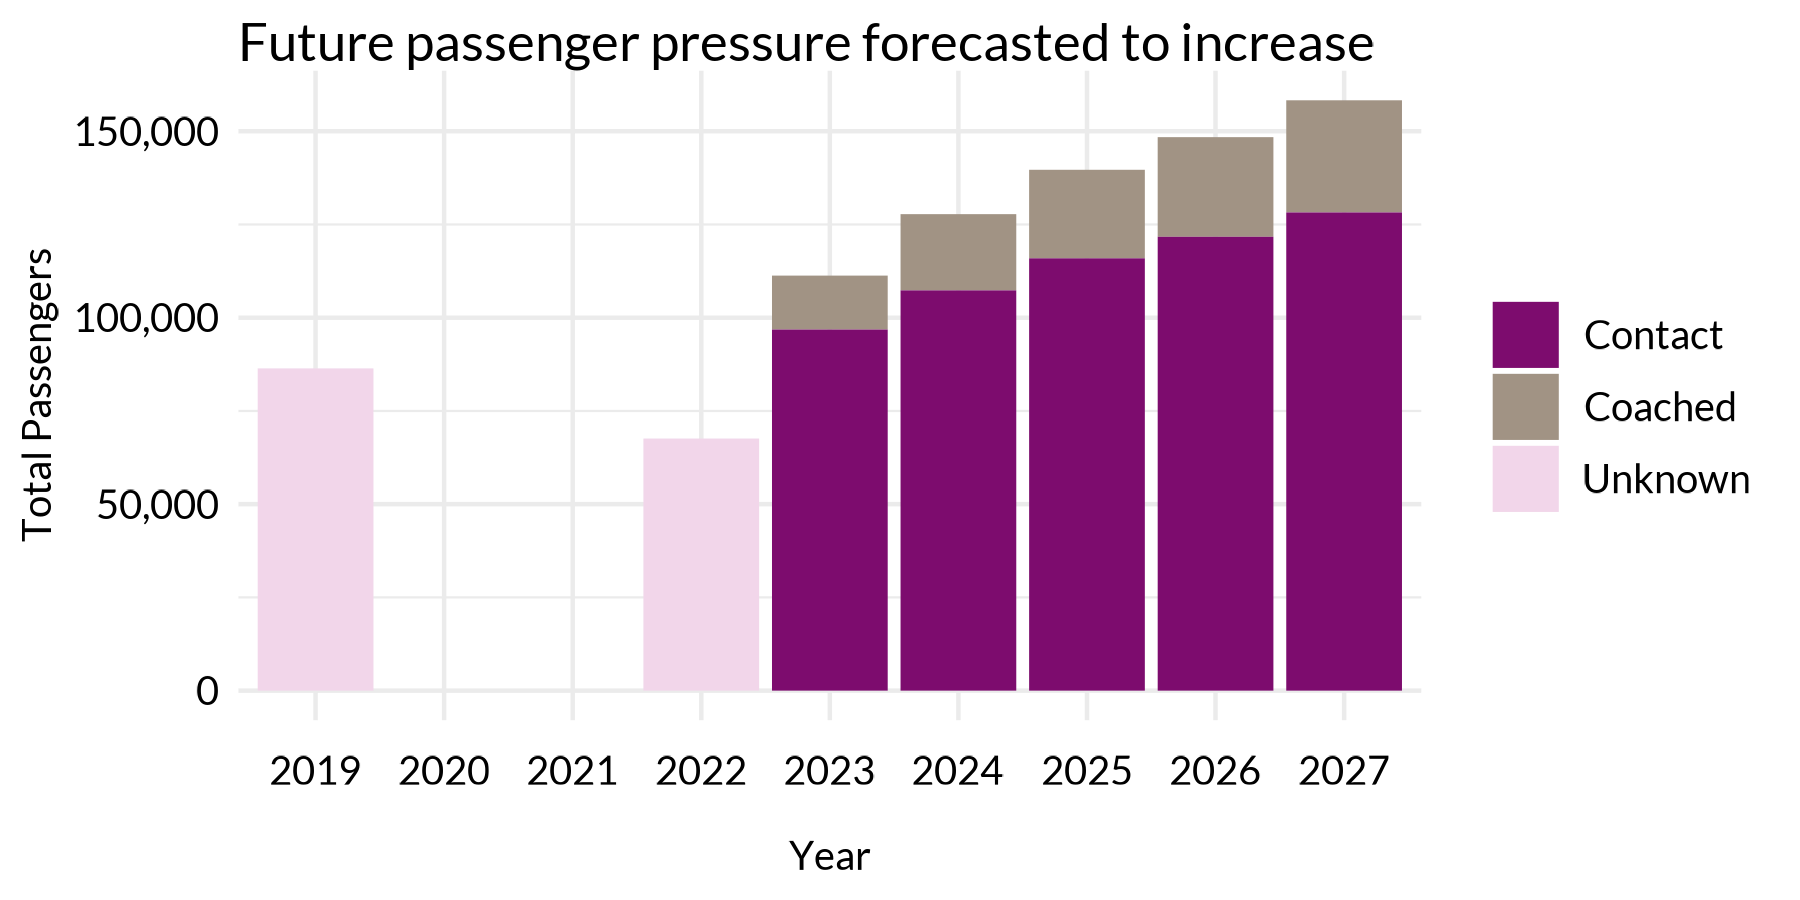
\includegraphics[width=0.8\textwidth]{figures/future_passenger_burden_fig.png}
     \caption{
     Historical and anticipated passengers arriving in Edinburgh Airport on international (non-UKIE) flights. For anticipated arrivals, passengers are split by route (coached vs contact).} \label{fig:future_passenger_burden}
\end{figure}

\subsection{External Data} \label{sec:observed_arrivals_data}

\paragraph{eGate uptake} 
The UK government's target for \gls{egate} \textit{uptake} (the proportion of eligible passengers choosing to use an \gls{egate}) has been set at 80\% \cite{UK_border_2025}, which was broadly met on a national level in 2019 and the first quarter of 2020. For airports in Scotland and the North of England the average uptake was lower, at around 70\% for the same period \cite{Inspection_eGates}. While there were no publicly available data for Edinburgh Airport, Glasgow Airport's uptake of around 60\% represents some of the lowest utilisation of \glspl{egate} nationwide \cite{Inspection_eGates}.

\paragraph{Average wait time at eGates}
The average wait time at \glspl{egate} at UK airports for the financial years 2017-18, 2018-19, 2019-20 and Q1 2020 was six minutes and one second \cite{Inspection_eGates}. Stansted and Luton reported averages just below three minutes. Glasgow Airport's average waiting time for \glspl{egate} was over 8.5 minutes. However, their calculation was based a shorter time period (December 2017, January 2018, and February 2019), and may therefore be unrepresentative \cite{Inspection_eGates}.


\paragraph{Historical arrivals data}
We accessed complementary historical flight arrivals data for more than 83,000 passenger flights from Edinburgh Airport Noise Lab \cite{noise_lab}. For these arrivals from the years 2019 to 2022, we were able to recover departure airport, aircraft type (and therefore approximate passenger count), and scheduled vs actual arrival times. This did not however include coached vs contact status, unlike our future arrivals dataset. 

% % latex table generated in R 4.2.3 by xtable 1.8-4 package
% Sun Apr 16 20:26:26 2023
\begin{table}[ht]
\centering
\begin{tabular}{cccc}
  \hline
{\textbf{Year}} & {\textbf{Start Date}} & {\textbf{End Date}} & {\textbf{Number of Flights}} \\ 
  \hline
2019 & 01/01 & 31/12 & 51,670 \\ 
  2020 & 01/01 & 31/12 & 15,376 \\ 
  2021 & 01/01 & 31/12 & 13,314 \\ 
  2022 & 01/01 & 31/12 & 31,983 \\ 
   \hline
\end{tabular}
\caption{Historical arrivals for Edinburgh Airport, 2019-2022. \label{tab:observed_schedule}} 
\end{table}


Aircraft type and maximum passenger capacity were established by cross-linking with another publicly available dataset \cite{aircraft_capacity}. The average percentage of occupied seats for a given flight ranged from 86\% in 2019 for international flights in the UK \cite{loading_factor_national} to self-reported 91\% for a budget airline in 2022 \cite{loading_factor_ryanair}.

\paragraph{Airport classification}
We assume that the passenger nationality split depends on departure airport, and therefore group airports into the following categories: 
\begin{itemize}
    \item \textbf{UKIE}: All airports in the United Kingdom (including Northern Ireland), the Crown Dependencies, and the Republic of Ireland.
    \item \textbf{EU+ hubs}: Hub airports in EU+. These are Amsterdam Schiphol (AMS), Atlanta International (ATL), Paris Charles de Gaulle (CDG), Dallas (DFW), Denver (DEN), Frankfurt (FRA), and Chicago O'Hare (ORD) \cite{mega_hubs}.
    \item \textbf{EU+ non-hubs}: Airports which are not hubs but are located in EU+.
    \item \textbf{Other hubs}: Hub airports outside of EU+. These are Dubai (DBX) and Istanbul (IST) \cite{mega_hubs}.
    \item \textbf{Other non-hubs}: Airports which are not hubs and are located outside of EU+.
\end{itemize}


\section{Methods} \label{sec:methods}

In this section we describe our methodology, including details of our abstract modelling framework, practical implementation, construction of a variety of demand scenarios, and system for evaluating \glspl{kpi}/\glspl{sla}.

\subsection{Passenger Processing Model}

    For all subsequent modelling we use a conceptual `passenger processing model' describing the steps an arriving international passenger experiences at Edinburgh Airport. Such a model is inherently a simplified view, but ideally chosen at a level of abstraction is nevertheless informative of real-world processes. Our passenger processing model consist of three steps, outlined below:
\begin{enumerate}
    \item \textbf{Aircraft}: Aircraft with passengers on board arrive at Edinburgh Airport. The aircraft taxi to their parking positions and their doors are opened. \label{step:aircraft}
    \item \textbf{Route}: Passengers make their way from their aircraft to the immigration hall, either by walking to the building (contact) or via a bus (coached). \label{step:route}
    \item \textbf{Immigration}: Passengers queue in the immigration hall and are processed at the border, either by a \gls{bfo} at a desk or at an automated \gls{egate}. \label{step:immigration}
\end{enumerate}
 We visualise the flow of information through our processing model in Figure~\ref{fig:PPM_threesteps}. We start with a dataset of arriving flights and generate a dataset of passengers (\textit{Aircraft} step). In the \textit{Route} step these passengers are then brought from the aircraft to the immigration hall. Finally, in the \textit{Immigration} step they queue up and are subsequently processed at the border.

\begin{figure}[!ht]
    \centering
    \figuretitle{Abstracting arriving passengers' flow through the airport}
    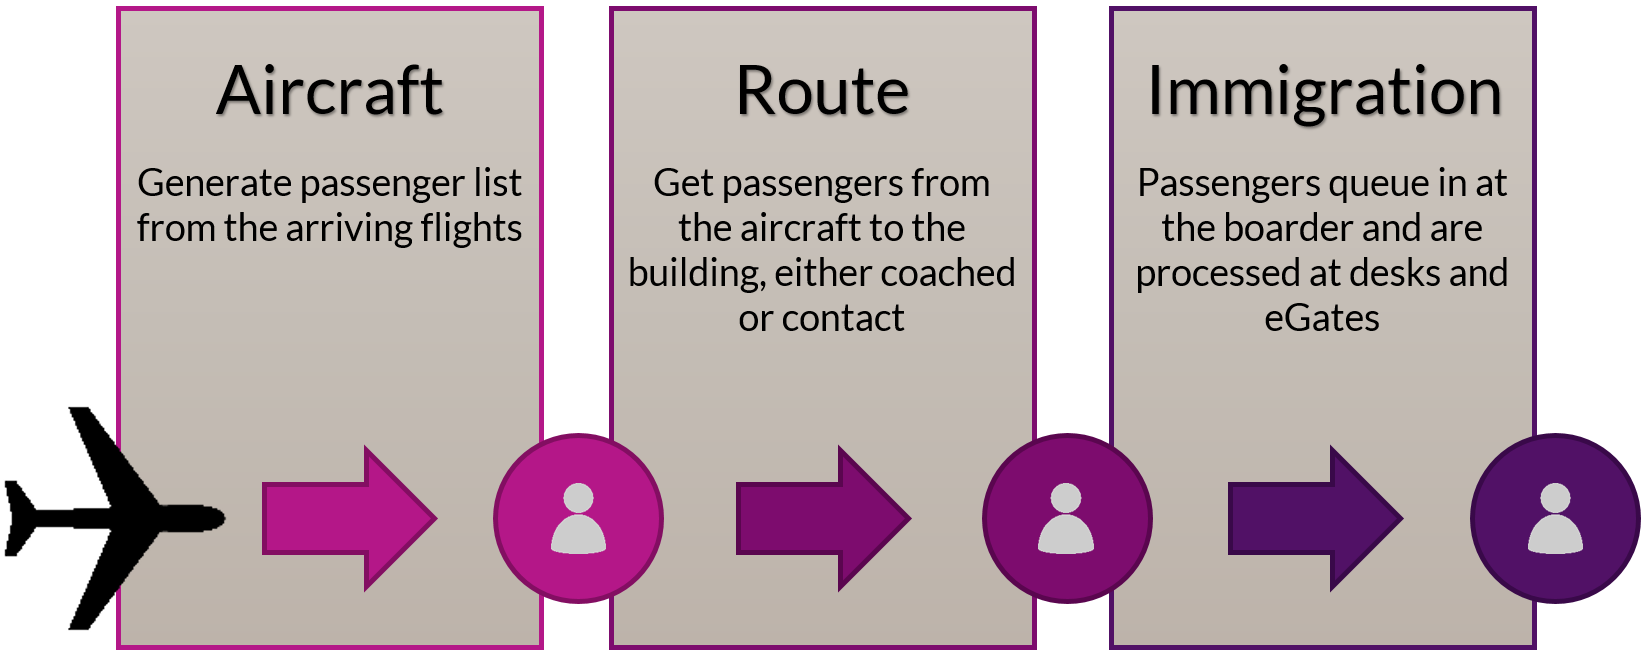
\includegraphics[width=0.7\textwidth]{figures/ThreeSteps.png}
     \caption{Three steps that make up the passenger processing model.} \label{fig:PPM_threesteps}
\end{figure}

\subsection{Assumptions and Choices}
% these are slightly different for competition and noise data
At each step of the Passenger Processing Model there are assumptions to be made and choices to be taken. We summarise them here. Our key parameters for robustness checks are the number of \glspl{egate}, \gls{egate} eligibility, and the \gls{egate} uptake, which are defined in Section~\ref{subsec:choices_immigration}.

\subsubsection{Aircraft}

\paragraph{Departing airport classification}
The arrivals dataset provided by the modelling competition (Section~\ref{sec:future_arrivals_data}) does not contain information regarding the departing airport. As this is provided in the additional dataset (Section~\ref{sec:observed_arrivals_data}) we are able to randomly sample airport classifications for the competition dataset conditional on the number of passengers on the flight, for an approximate distributional match. 



% \paragraph{Number of passengers}
% The competition dataset contains the number of passengers on board each flight. This information is not available for the additional historical data, but can be simulated with the aircraft type, its maximum capacity, and the load factor. \jbnote{Do we need to choose an overall load factor? Also slightly unsure if we'll ever actually ever need this simulated on historical data.} \bdnote{we use it indirectly to simulate an airport classification as the load factor goes into the historical quantiles. Could also be ignored.}

\paragraph{Coached vs contact}
The competition data gives an overall split of flights that are coached or contact for each year. We assume that the decision between coached or contact is independent of all flight characteristics. Anticipated future coached vs. contact splits are shown in Figure~\ref{fig:future_passenger_burden}, with coached arrivals continuing to form a minority, albeit an increasing one, of future aircraft arrivals.


\subsubsection{Route}

\paragraph{Arrival profile} 
 Passengers  brought to the immigration hall coach arrive at the queue in rapid succession. Coached passengers arrive at the immigration queue on average every 1 second. Contact passengers make it to the immigration queue every 5 seconds.

\paragraph{Coach availability}
For this analysis we assume sufficient coaches are always available to transport passengers from the aircraft to the airport building. While this might not be always the case, it provides us with a ``worst case'' scenario from the perspective of the immigration hall, which is most interesting for us. Any delay in passengers due to unavailability of coaches would smooth out peaks.

\subsubsection{Immigration} \label{subsec:choices_immigration}

\paragraph{Number of eGates and desks} There are currently 10 \glspl{egate} and 9 \gls{bfo}-staffed desks in use at Edinburgh Airport. In our analysis we simulate the effects of an increasing number of \gls{egate}.



\paragraph{eGate eligibility}
As only passengers from certain countries are can use \glspl{egate}, we make the percentage of passengers eligible for \glspl{egate} per aircraft dependent on the classification of the airport. For example, we assume that an aircraft from a hub is more likely to carry a variety of international passengers, of which fewer can use \glspl{egate} compared to a flight from a EU+ non-hub. 

\paragraph{eGate uptake} 
Not all passengers who are eligible to use eGates choose to do so for a variety of reasons. As a base case we use a 70\% uptake, which is selectively increased in our simulation. 


\paragraph{Priority for failed eGate passengers}
Passengers who used an \gls{egate}, but failed to use it successfully, need to exit the \gls{egate} back into the immigration hall to complete their immigration at a staffed desk. They join a separate queue towards the desks, which is located next to the general desk queue. Whenever a desk can handle a new person, priority is given to the passenger from the failed \gls{egate} queue with a probability of 75\%.

% \paragraph{Capacity split}
% Which percentage of the hall capacity is allocated to the desk queue. Varied to change the effect of queue length of contingency usage.
% Note that we can't split the other areas

\subsection{Implementation}

We now describe how we process competition datasets to calculate \glspl{kpi} under different simulation scenarios. Figure~\ref{fig:workflow_fig} gives an illustration of our workflow for a two-hour window of anticipated arrivals. 
\begin{figure}[!ht]
    \centering
    \figuretitle{Implementation of passenger processing model allows for systematic simulation of immigration queues}
    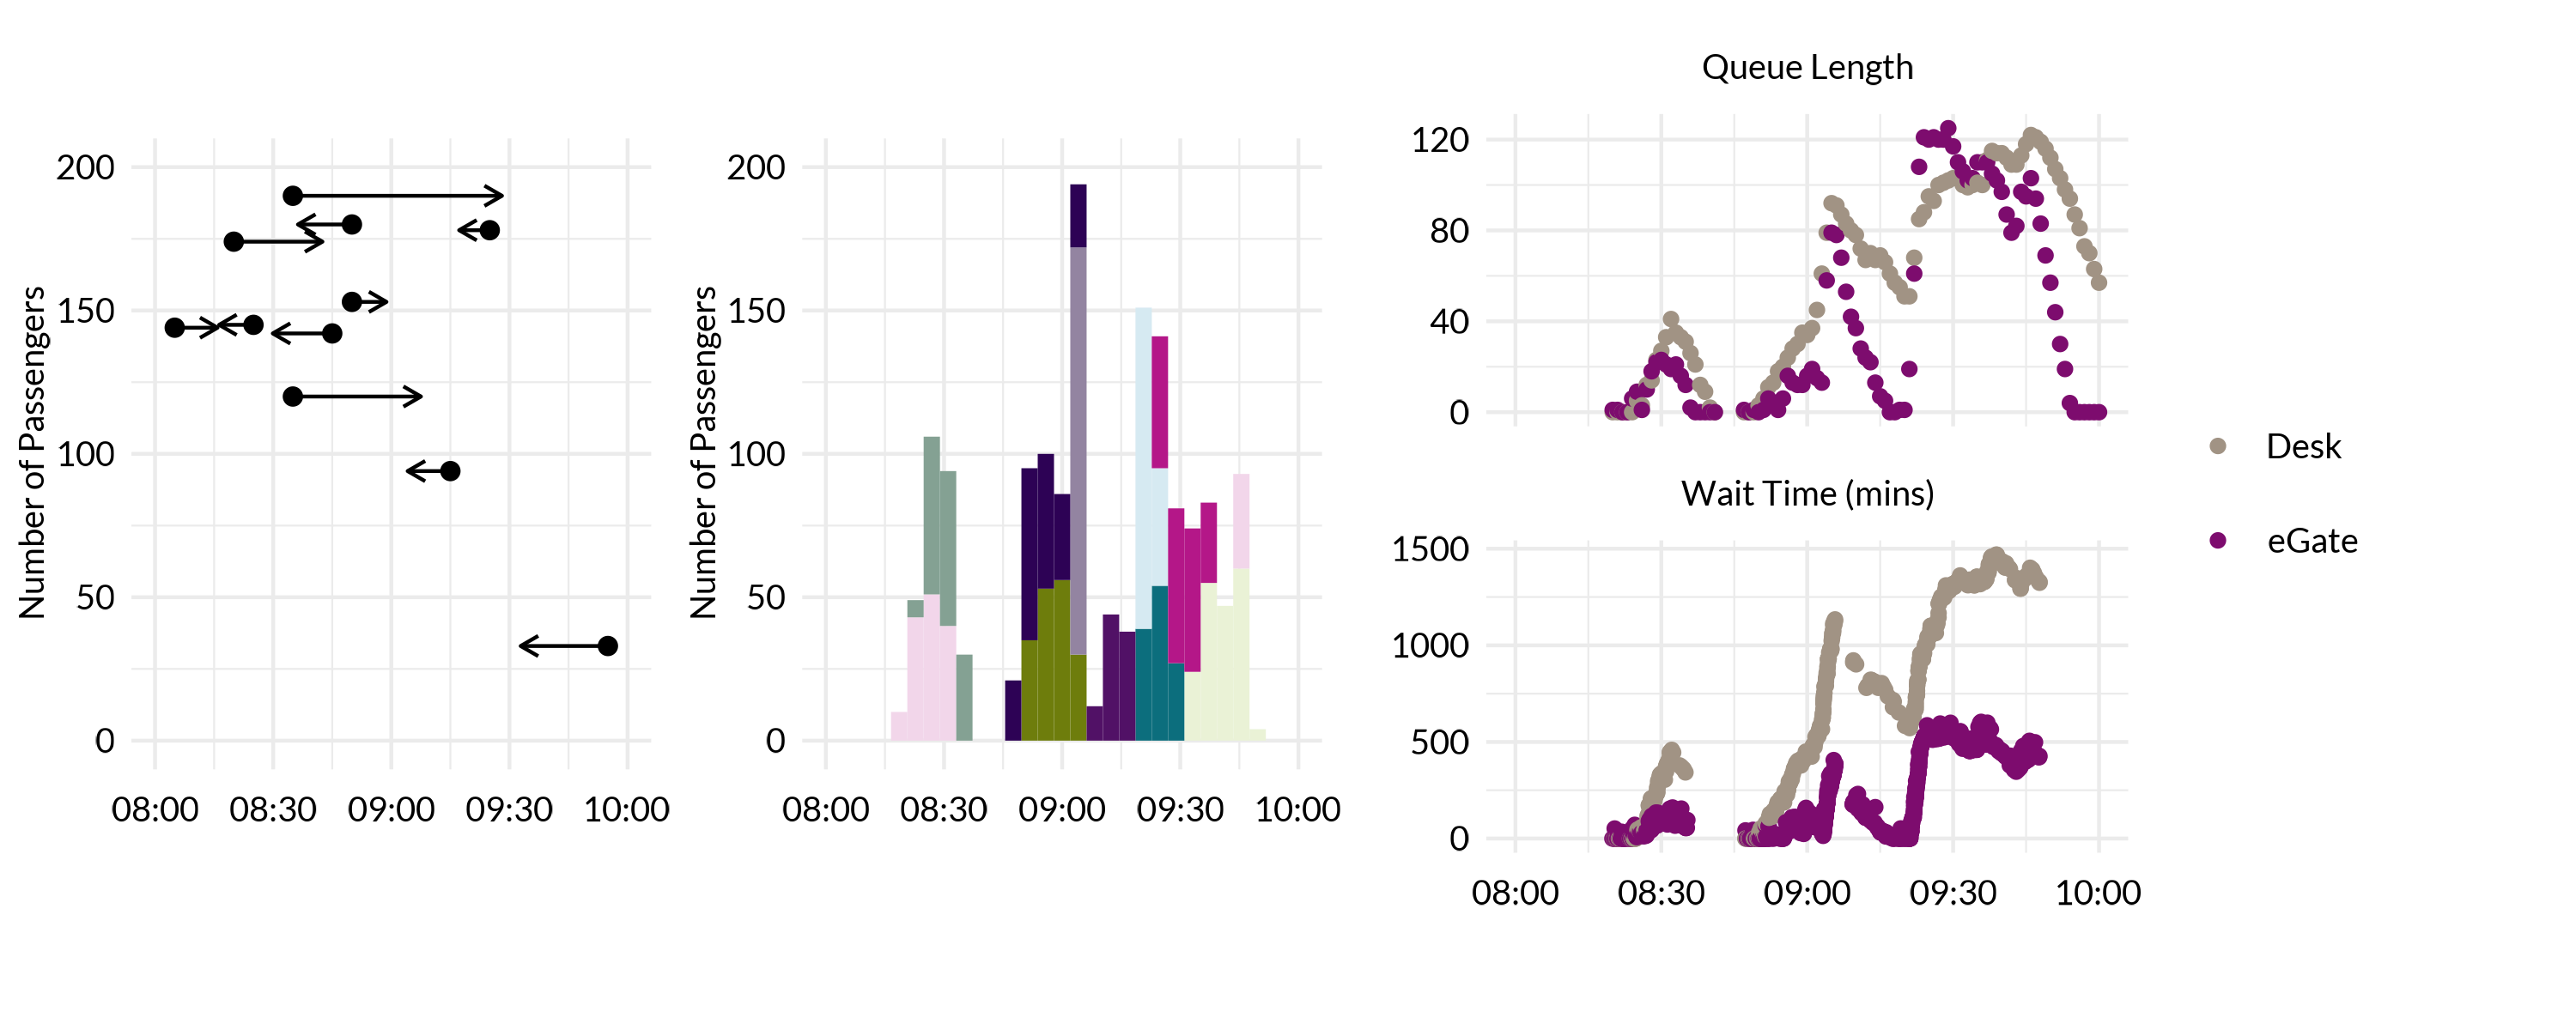
\includegraphics[width=1.1\textwidth]{figures/workflow_fig.png}
    % \vspace{-5pt}
     \caption{Example application of simulation workflow for three-stage passenger processing model, applied to anticipated arrivals schedule between 08:00am and 10:00am on the 11th of June, 2023. \textbf{Left}: Aircraft of different sizes arrive at Edinburgh Airport. Arrows from scheduled to actual arrival time. \textbf{Centre}: Passengers disembark from their aircraft and are coached or walk via contact to to immigration hall. Passenger count is coloured by flight. \textbf{Right}: Passengers queue, either for a desk border check or an \gls{egate}. Queue length is reported every minute (upper panel), and wait time from arrival in the immigration hall to the start of the relevant border check (lower panel).} \label{fig:workflow_fig}
\end{figure}
\subsubsection{Aircraft}
We take the provided flight schedule data as an input of the Aircrafts step. We assume that all of the flights provided are coming from non-UKIE destinations and hence their passengers need to clear immigration at Edinburgh Airport. Based on the flight schedule we simulate the actual arrival according to the given delayed/early arrival information. Given the provided split per year we decide at random for each flight if it is coached or contact. Based on this we sample a base route time from the parking position. The passenger numbers per flight are known, and we use this information to sample a departure airport classification according to the empirical distribution obtained from the historic flight data.

Taking the above flight information as an input we generate a list of passengers per flight. For each passenger we sample a nationality classification based on the departure airport. The output of the Aircraft step is a passenger list, which also contains all the covariates describing their flight.

\subsubsection{Route}

Given the passenger list from the previous step, we simulate the time each passenger spends getting from their flight's parking position and to the immigration queue. This is depending on the base route time 
of the flight and whether they were on a coached flight or not.

This step adds additional information to each passenger. Crucially, it gives us the arrival time of each passenger at the immigration queue. 

\subsubsection{Immigration}

Based on the passenger-level information obtained in the previous step we now process each passenger at the border according to their arrival time at the immigration queue. First, we determine the eligibility to use \glspl{egate} per passenger according to their nationality classifications. 

Passengers not eligible to use \glspl{egate} join the desk queue and, once they reach the front of the queue and a free desk becomes available, they are processed by a \gls{bfo}. We sample the processing time for each passenger such that the transaction times match the provided information. Once a passenger is processed at a desk they have passed immigration and leave the system.

Not all passengers eligible to use \glspl{egate} will do so. The decision to use \gls{egate} is taken for each passenger according to the chosen \gls{egate} uptake rate. \gls{egate}-eligible passengers who choose to use a desk instead join the desk queue and are processed like any other passengers in that queue. 

Those who are eligible to use \glspl{egate} and choose to do so join the \gls{egate} queue. Once a passenger reaches the front of the queue and a free \gls{egate} becomes available they step into the \gls{egate} and are processed according to the provided transaction time. Most passengers finish this process successfully and exit the \gls{egate} on the other side, which completes their immigration and they exit the system.

A small fraction of passengers does not pass the \gls{egate} successfully. They are prompted to step out of the \gls{egate} back into the hall and have not completed immigration yet. Instead, they need to be processed by a \gls{bfo}. For that, these passengers are directed towards a separate queuing area in the middle of the hall that brings them towards the front of the desk queue. When a desk becomes available passengers that have failed the \gls{egate} have priority over the passenger at the front of the desk queue with a defined probability. Once they reach a desk, they are processed like any other passenger from the desk queue and exit the system.



\section{Recommendation}

Based on the methodology described in Section~\ref{sec:methods} we have simulated a variety of scenarios. There are three key parameters that we vary across simulations (1) the number of \glspl{egate}, (2) the \gls{egate} eligibility, and (3) the \gls{egate} uptake. This now allows us to make recommendations for the appropriate number of \glspl{egate} to cope with future demand on border operations at Edinburgh Airport. Robustness considerations are subsequently undertaken in Section~\ref{sec:robustness}. 

\subsection{Number of eGates} \label{sec:rec_num_egates}

The lowest feasible number of \glspl{egate} is of interest to Edinburgh Airport. Based on our extensive simulations we recommend the \gls{egate} strategy outlined in Table~\ref{tab:core_recommendation}, where for each year we give the minimum recommended number of \glspl{egate} to be available by that year (including currently available \glspl{egate}). 


% latex table generated in R 4.2.3 by xtable 1.8-4 package
% Thu Apr 27 17:58:27 2023
\begin{table}[ht]
\centering
\begin{tabular}{ccccc}
  \hline
{\textbf{2023}} & {\textbf{2024}} & {\textbf{2025}} & {\textbf{2026}} & {\textbf{2027}} \\ 
  \hline
 14 &  18 &  21 &  26 &  30 \\ 
   \hline
\end{tabular}
\caption{Core recommendation for eGate construction. \label{tab:core_recommendation}} 
\end{table}

% \begin{table}[!htp]
%     \centering
%     \begin{tabular}{cccccc}
%          2023 & 2024 & 2025 & 2026 & 2027  \\ \hline
%           x & x & x & x & x
%     \end{tabular}
%     \caption{Recommended Number of \glspl{egate} in operation each year.}
%     \label{tab:recommendation}
% \end{table}

This strategy has been chosen such that 99\% of \gls{egate} passengers wait less than an hour for every year in the given period \jbnote{and that contingency usage is never caused by \gls{egate} queues}, under the assumptions of eligibility and uptake shown in Figure~\ref{fig:core_rec_fig}. Following this strategy, the number of \gls{egate} passengers waiting for less than Edinburgh Airport's ambitious fifteen minute target is always above 75\%, and increases year-on-year. 

Without changes to \gls{egate} eligibility and uptake, no amount of \gls{egate} construction will alleviate some pressure on Edinburgh Airport's desk border check queues. In the simulations shown we have assumed smooth transitions in \gls{egate} eligibility and usage leading to the airport's 95\% total usage target by 2027 (see Section~\ref{subsec:choices_immigration}; bottom left panel of Figure~\ref{fig:core_rec_fig}). In this scenario, desk queue times (centre panel of Figure~\ref{fig:core_rec_fig}) are substantially lagging, and most concerningly extensive use is made of contingency capacity and even beyond contingency due to queues for desk border checks. 


\begin{figure}[!ht]
    \centering
    \figuretitle{Under core recommendation, eGate queue lengths and wait times meet SLAs}
    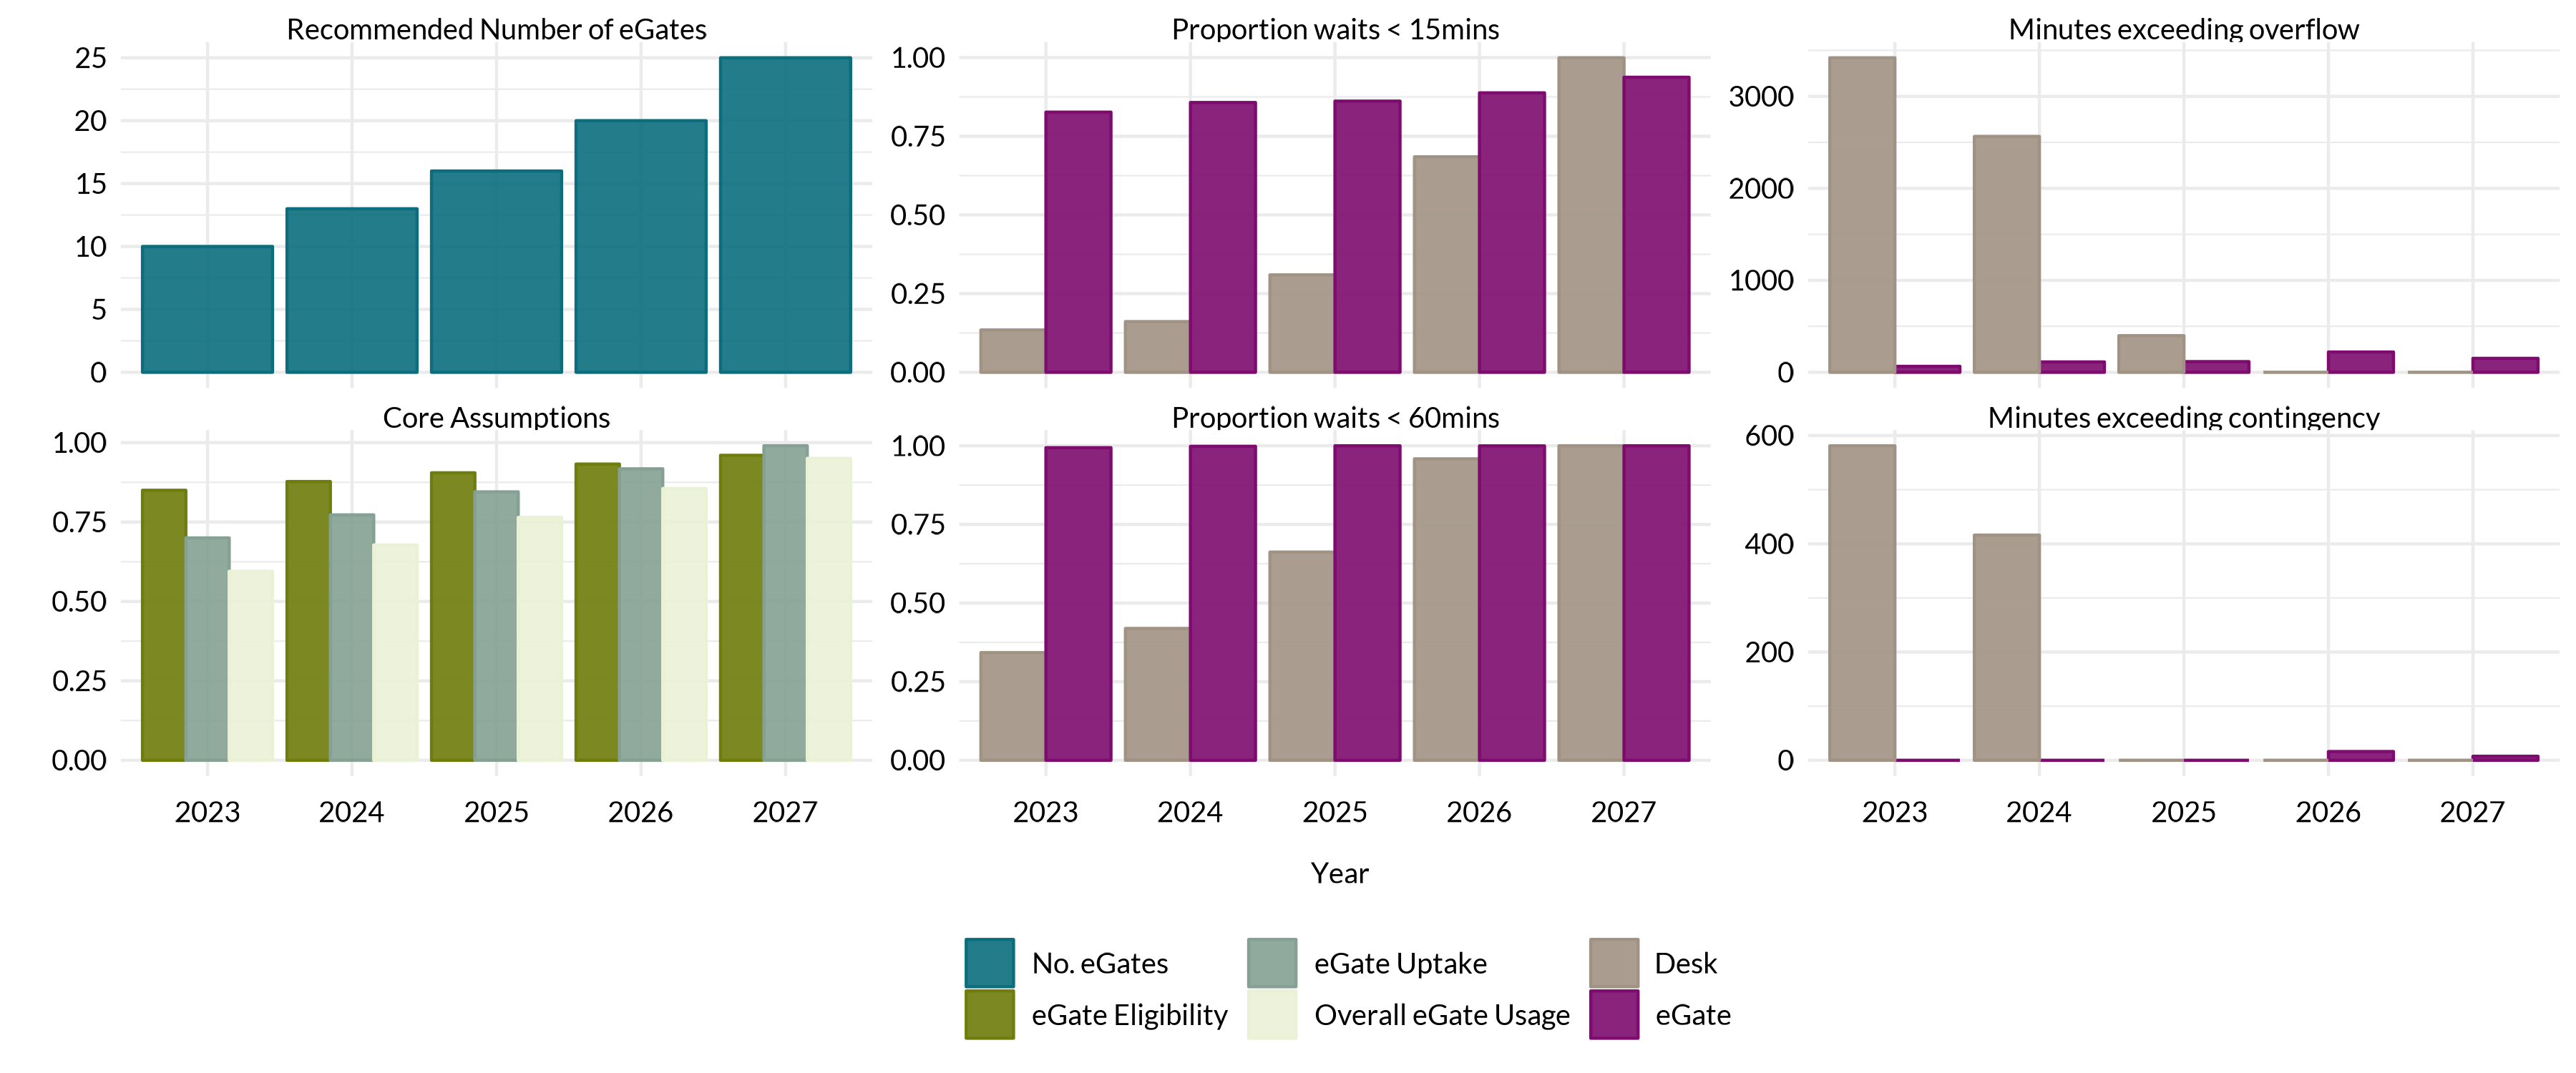
\includegraphics[width=\textwidth]{figures/core_rec_fig.png}
     \caption{\textbf{Left}: Core \gls{egate} construction recommendation and assumed progression of \gls{egate} eligibility and uptake. \textbf{Centre}: Wait time \glspl{kpi}, averaged over 100 simulations. \textbf{Right}: Queue length \glspl{kpi}, averaged over 100 simulations.} \label{fig:core_rec_fig}
\end{figure}

This recommendation results in an average wait time for \glspl{egate} between XX minutes (in 20XX) and XX minutes (in 20XX). This is higher than/lower than/in line with historic waiting times across the UK. It is higher/lower than Stansted and Luton, which reported particularly low figures, and higher/lower than Glasgow Airport, which reported some of the longest wait times. 

The number of recommended \glspl{egate} is to be understood as the number of \glspl{egate} required to be in operation. If maintenance and unplanned disruption exceed the historically low level \cite{Inspection_eGates}, this needs to be taken into account. Our recommendation implies the purchase of a total XX new \glspl{egate}, as there are currently 10 \glspl{egate} in operation at Edinburgh Airport. To put this number into perspective, the Home Office has approved funding of up to 70 \glspl{egate} UK-wide to increase capacity at larger airports \cite{Inspection_eGates}. With Edinburgh being among the top ten busiest airports in the UK \cite{busiestairport}, it does not seem unreasonable to assume that XXX new \glspl{egate} are built over the course of five years. 


\subsection{Hall Layout}
The \gls{sla} considers a total queue length. However, the queue space for desk and \glspl{egate} is separated by dividers, which are typically not moved. We therefore need to consider the given split of the hall space to accurately access whether the queue reaches outside of the hall. This is the case if either queue exceeds its allocated space, not just if the number of people in the queue increases beyond 500. 

Given the assumed number of \gls{egate} eligibility and uptake, and our recommended number of \glspl{egate} as outlined in XXXX, the optimal capacity split to minimise queuing outside of the immigration hall is allocating XXX to the desk queue and XXX to the \gls{egate} queue.
 

\section{Robustness Considerations} \label{sec:robustness}
In producing the recommendation given Section~\ref{sec:rec_num_egates}, we made assumptions about external factors such as \gls{egate} eligibility and the progress of \gls{egate} construction that could be liable to change. Here we investigate the effect of such changes on the performance of immigration services.

\subsection{Eligibility and Uptake}
Edinburgh Airport envisages 95\% of passengers using \glspl{egate} by 2027, up from 60\% at present. To a first approximation, overall \gls{egate} usage is equal to the product of \gls{egate} eligibility and uptake. While increases in \gls{egate} eligibility are planned \cite{UK_border_2025}, they fall largely outside of Edinburgh Airport's direct control. We therefore aimed to test whether lower than anticipated \gls{egate} eligibility could be compensated for by improvements to \gls{egate} uptake. We therefore simulated a variety of combinations of eligibility and uptake for arrivals in 2027, the busiest year forecast in the given time period. In Figure~\ref{fig:robustness_fig} we show a selected range of \glspl{kpi} for these scenarios, and see that as long as eligibility reaches 90\% comparable performance is achievable purely through compensatory improvements in uptake.

\begin{figure}[!ht]
    \centering
    \figuretitle{Under misspecification of eGate eligibility, increased eGate uptake can provide balance}
    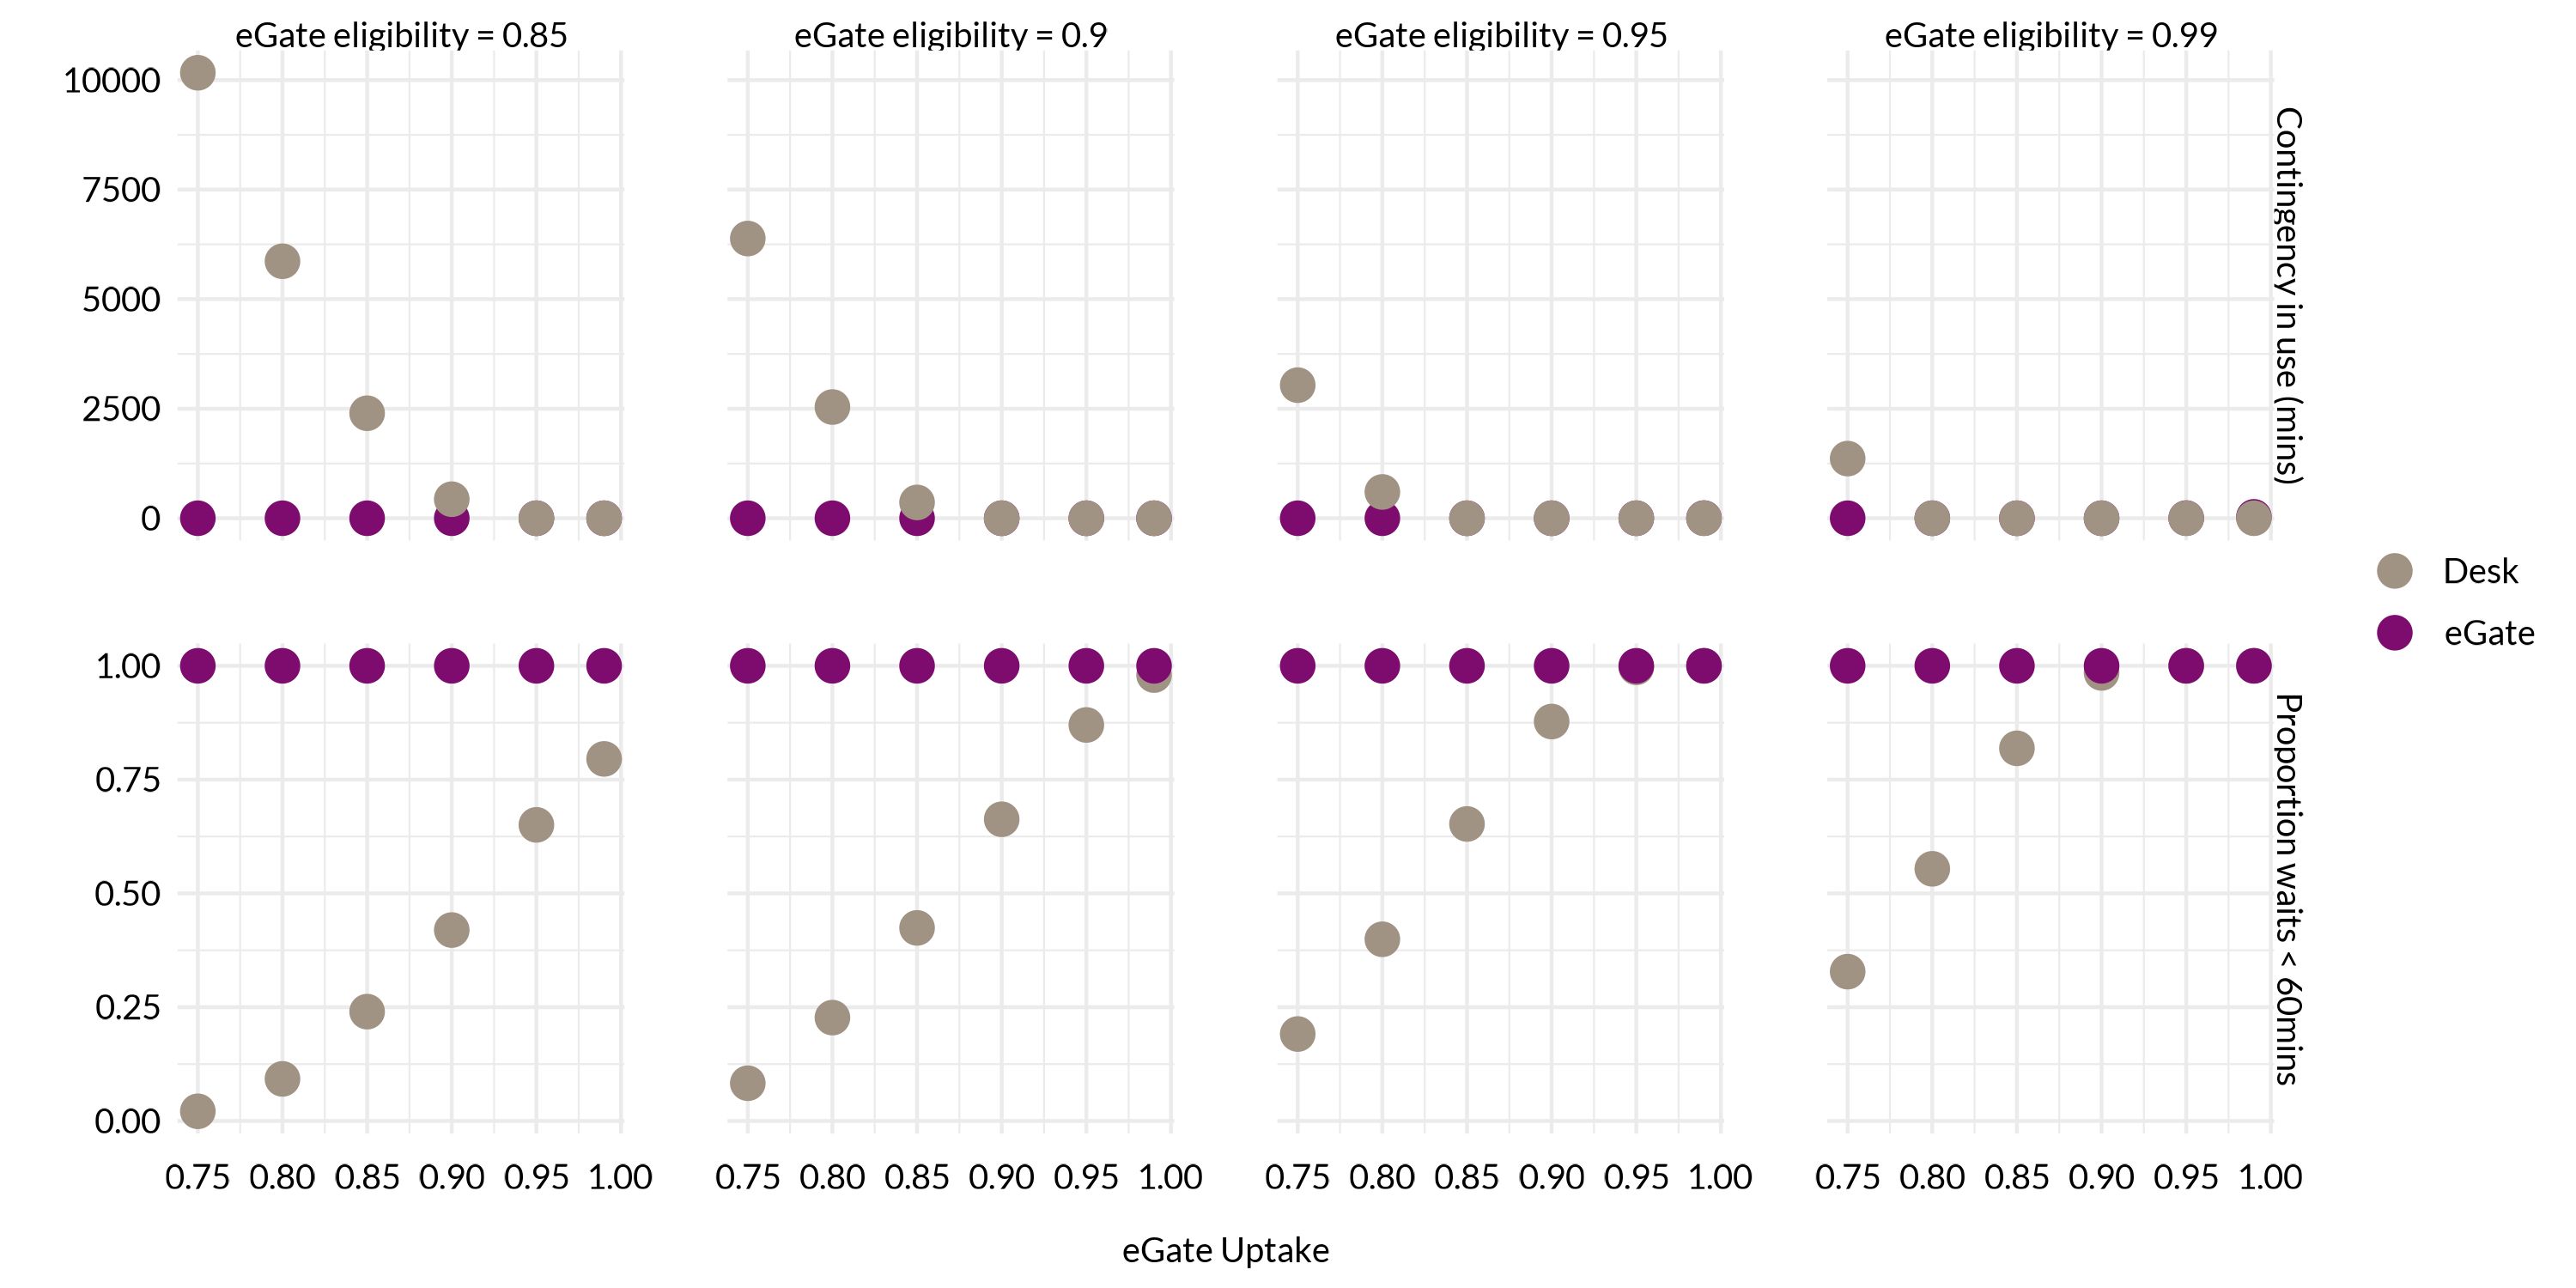
\includegraphics[width=\textwidth]{figures/robustness_fig.png}
     \caption{\textbf{Top panels}: Average (over 100 simulations) number of minutes in 2027 week spent with contingency use caused by \gls{egate} or desk queues, under a variety of eligibility/uptake scenarios. \textbf{Bottom panels}: Average (over 100 simulations) proportion of passengers waiting less than 60 minutes, for the same range of scenarios.} \label{fig:robustness_fig}
\end{figure}

\subsection{Number of eGates}
We selected the recommendation laid out in Section~\ref{sec:rec_num_egates} in order to minimise the need for new \gls{egate} construction while satisfying the conditions we described. However, for practical reasons the airport may choose to place immigration services under stress for a short period in order to construct more \glspl{egate} at once. It is also possible that \glspl{egate} may fail or be delayed in construction. In Figure~\ref{fig:minus_core_rec_fig}, therefore, we present identical analytics to Figure~\ref{fig:core_rec_fig} for a `recommendation-minus-one' strategy, whereby for each year after 2023 (in 2023 we do not recommend construction of new \glspl{egate}) we consider one fewer total available \glspl{egate} than were recommended.

\begin{figure}[!ht]
    \centering
    \figuretitle{With one fewer eGate than recommended, queue length SLAs are breached}
    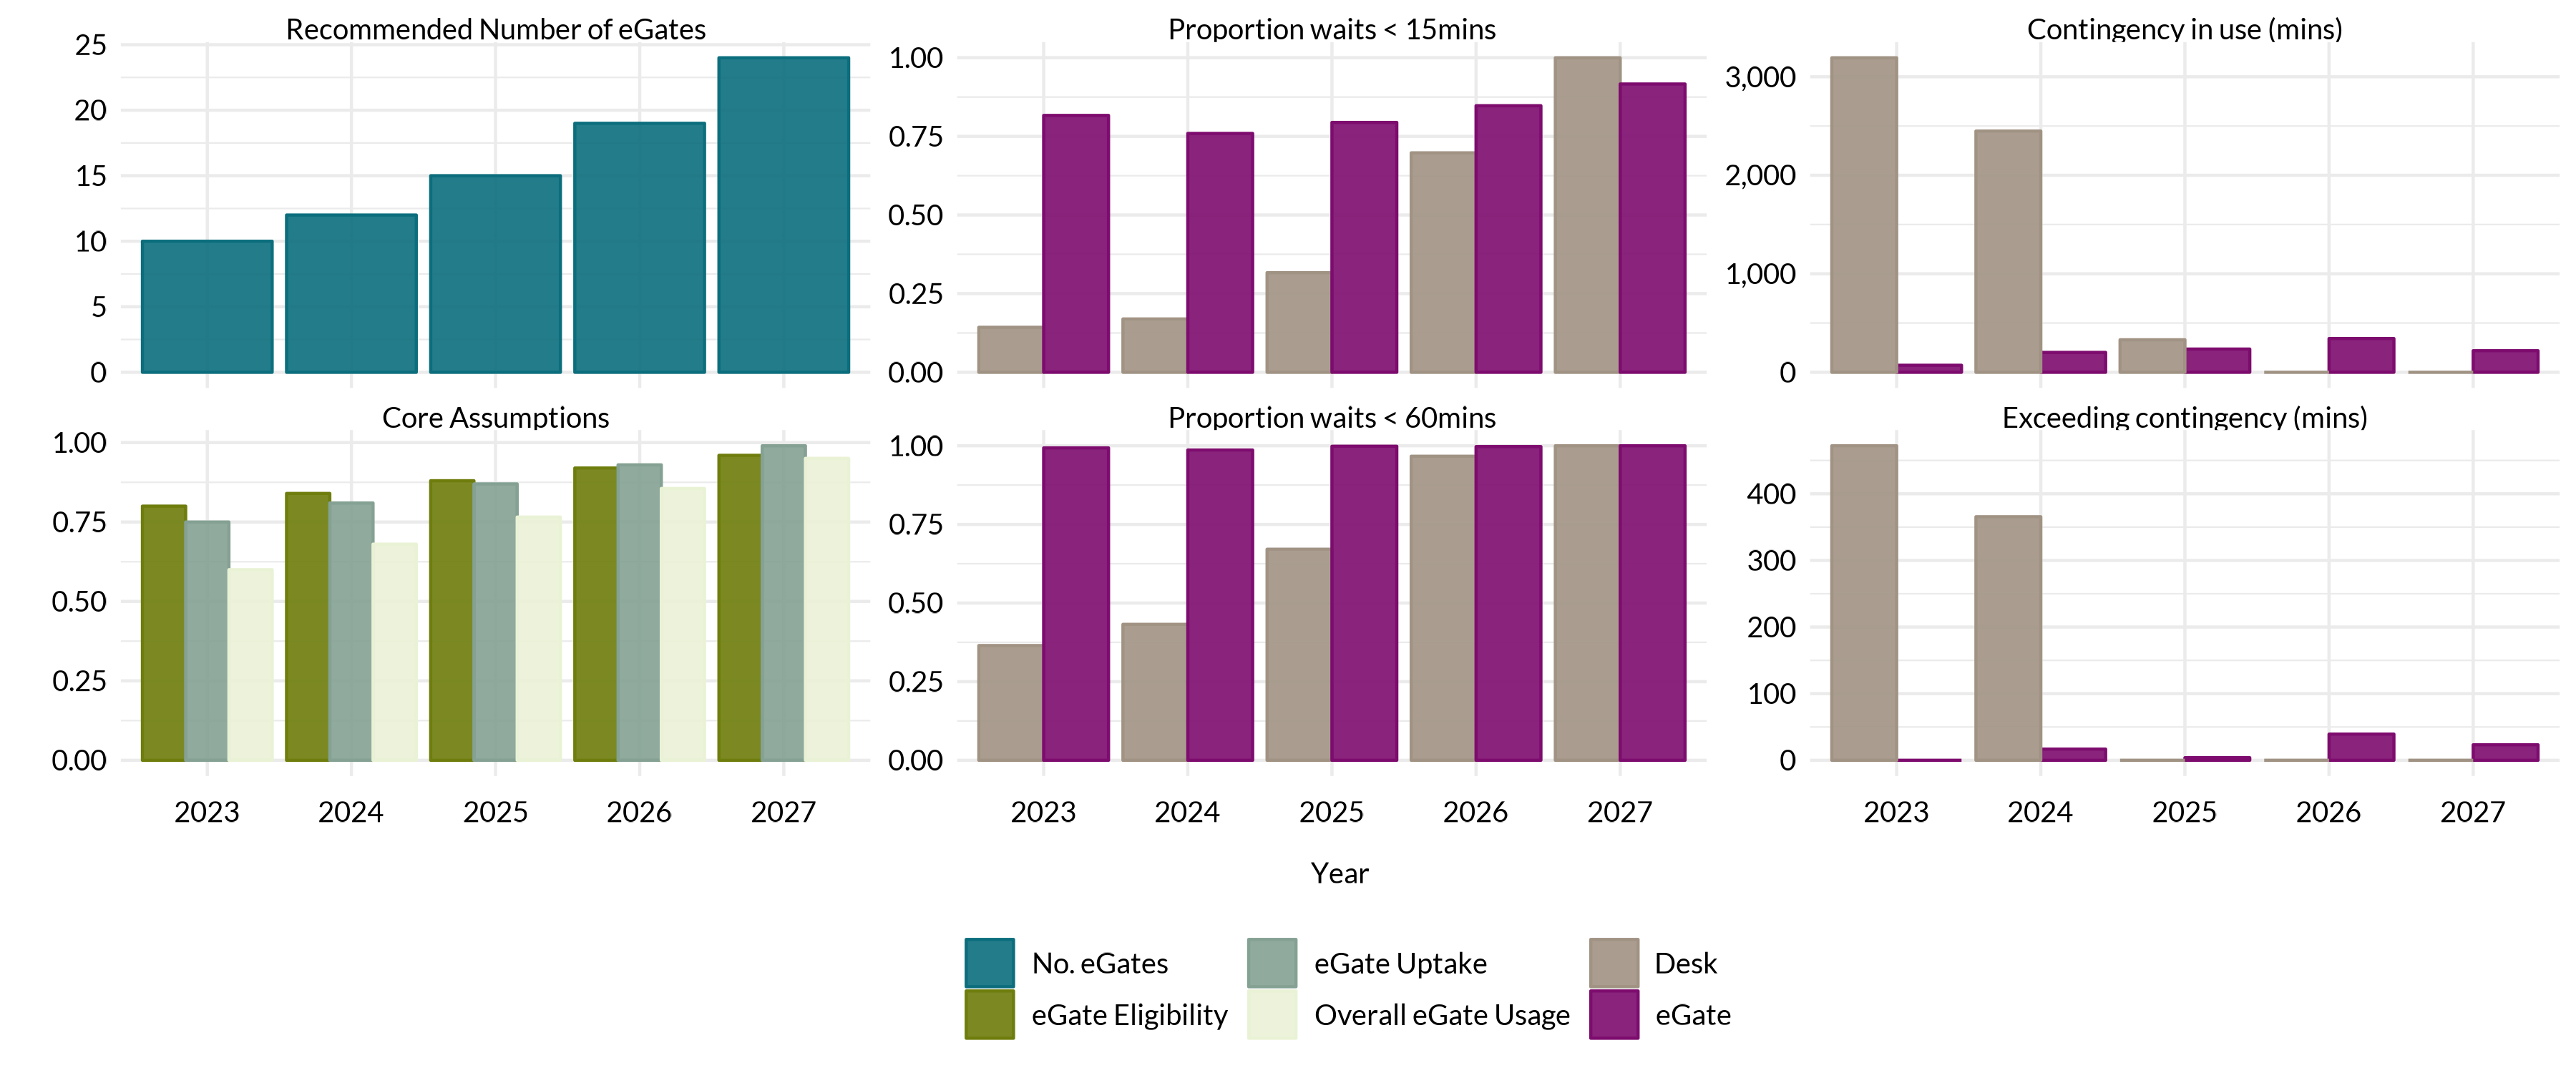
\includegraphics[width=\textwidth]{figures/minus_core_rec_fig.png}
     \caption{\textbf{Top Left}: Adjusted \gls{egate} construction schedule, with one fewer \glspl{egate} than recommended for each of the years 2024-2027. \textbf{All other panels}: as in Figure~\ref{fig:core_rec_fig}.} \label{fig:minus_core_rec_fig}
\end{figure}

\section{Conclusions}
Edinburgh Airport has identified strain on immigration services due to increased passenger burden as a risk to border operations over the next five years. To address this, they have asked for a simulation model to test different demand scenarios and process enhancements. We have developed such a model, which can be explored interactively via a \href{https://github.com/cobrbra/immigration_queue_simulation_edinburgh_airport}{Shiny App}. We have incorporated data provided by the modelling competition and external sources to guide simulation parameters. Where we could not find appropriate data sources, we have made assumptions erring towards pessimistic values in order to evaluate worst-case scenarios. We have provided a central recommendation for the construction of X, X, X, and X new \glspl{egate} by 2024, 2025, 2026, and 2027 respectively. From extensive simulation and robustness analyses, our key conclusions are sumarised below.

\begin{tcolorbox}[
colframe=edi-dark-purple,
colback=edi-light-purple,
fonttitle=\bfseries,
title = {Summary of Key Conclusions}]
\begin{enumerate}

    \item \textbf{Building five or fewer \glspl{egate} per year can keep \gls{egate} queue \glspl{kpi} within appropriate levels.}\\
    Our recommended schedule for \gls{egate} construction never exceeds one comprising five new \glspl{egate} per year, and allows for consistent satisfaction of UK Border Force's one hour target and sustained improvements towards satisfying Edinburgh Airport's aspirational 15 minute target for \gls{egate} passengers. Alternately, practical constraints may motivate building all new \glspl{egate} in one go. Such scenarios can easily be explored in our \href{https://github.com/cobrbra/immigration_queue_simulation_edinburgh_airport}{Shiny App}. \\ 
    \item \textbf{Regardless of new \glspl{egate}, long desk queues pose a serious risk until \gls{egate} usage increases.}\\
     Additional \glspl{egate} need to be used in order to have a positive impact on border operations. To that extend it is important that \glspl{egate} usage is high as soon as there is sufficient \gls{egate} capacity to match. The airport's current estimate of overall \gls{egate} usage is 60\% \cite{modelling_competition}. At this level, the passenger arrivals schedule proposed for July 2023 implies sustained periods with desk queue lengths severely compromising immigration services, regardless of \gls{egate} installation numbers.\\
    
    \item \textbf{Effective \gls{egate} usage may be achieved by expanded eligibility or by increased uptake.}\\
    Under high demand scenarios (such as those anticipated by 2027), high \gls{egate} usage is required. Increased eligibility is expected, but broadly outside the airport's control. Improvements to uptake, however, may be achieved with clear and prominent signage and direction. Flow hosts at \glspl{egate} may also play a critical role (as suggested in \cite{Inspection_eGates}, paragraph 6.28: ``[flow hosts are]... particularly vital given high passenger usage and rapid throughput'') in directing passengers.\\
    
    \item \textbf{Lower-than-recommended \gls{egate} construction will impact queue lengths before wait times.}\\
\end{enumerate}
\end{tcolorbox}


\subsection{Future Work}
Many options for modelling lay beyond the scope of this report (and so are omitted) but may provide avenues for further work. We list several here, some of which incorporate modelling considerations relating to other airport teams (e.g. operations, aeronautics) and may therefore provide opportunities for future collaboration.

Throughout our analyses we have assumed aircraft delays to occur independently. In practice, delays are highly interrelated, as well as being associated with weather and air traffic control operations.

In 2019, 55\% of all flights arriving at Edinburgh Airport came from UKIE airports \cite{noise_lab}. It is currently unclear whether domestic air travel will become less popular, with any future trends depending on government policy \cite{flight_tax_independent}, post-Covid travel habits \cite{post_covid_flights}, and competition from other infrastructure including rail \cite{train_airplane_guardian}. If Edinburgh and other airports shift to more non-UKIE flights, demand on border operations would continue to change in complex ways. For example, while overall passenger burden might increase, logistical simplifications could be possible with reduced need to provide separated routes for domestic and international arrivals.

Demand for contact stands for aircraft at Edinburgh Airport is expected to increase with arrivals, in particular increasing arrivals of aircraft with large wingspans and/or retrofitted winglets (which may take up two stands). Site footprint restrictions make the construction of new contact stands unlikely. Future arrivals could therefore skew more strongly towards coached flights. While this is reflected in the modelling assumptions provided here, future work might incorporate operational factors to understand under what circumstances coached arrivals are most likely to be more predominant (e.g. later in the day). 

We have modelled a fixed number of nine desk border checks located in one immigration hall throughout all of our analyses. In reality, Edinburgh Airport has access to two immigration arrivals buildings (International Arrivals 1 and International Arrivals 2), the former of which is only opened at certain times. Future work might investigate optimally scheduling the opening of IA1.

Finally, in our analysis we have simulated `normal' border operations. This excludes special cases, such as \glspl{bfo} deciding to close all \glspl{egate} for selected high-risk flights \cite{Inspection_eGates}. 

\newpage
{\footnotesize
\bibliography{report/references}}
% \bibliography{report/references.bib}

\end{document}